\section{Inledning}
Den här designspecifikationen är menad att noggrant specificera hur det system som beskrivs i projektets kravspecifikation skall konstrueras. Detta system skall kunna följa en bana enligt figur 1 där det skall kunna plocka upp och sätta ned paket på de utsatta stationerna B och C. Det skall även kunna detektera och hantera avbrott i banan (A) samt slutstationer (D). 

\begin{figure}[h]
\center
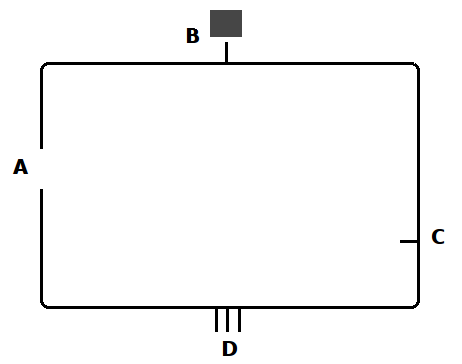
\includegraphics[scale=0.4]{figur}
\caption{Banöversikt} \label{systemskiss:banoversikt}
\end{figure}